\documentclass{jhwhw}
	\usepackage{enumitem}
	\usepackage{soul}
	\usepackage{float}
	
	\title{EE 4341 Homework 1}
    \author{Alex Biedny}
    \date{\today}
    \chead{EE 4341 Homework 1}
    \lhead{Alex Biedny}
    
\usepackage{graphicx}
\begin{document}

\maketitle

\problem{}
\begin{enumerate}
\item With no bypassing, it will take 9 instruction cycles to completely execute both instructions. This is because the value of $t2$ will not be available until after the first instruction finishes the W stage, meaning the second isntruction cannot start executing until the first instruction is in the W stage.
\item With bypassing, it will take 6 instruction cycles to completely execute both instructions, becuase the value of $t2$ will be ready right after the E stage of the first instruction.
\end{enumerate}

\problem{}
\begin{enumerate}
\item Memory region: KSEG1\\
Physical addr of instruction: 0x00000028\\
Type: Boot flash \\
Registers: sp = r29
\item Memory region: KSEG0\\
Physical addr of instruction: 0x00000108\\
Type: Program flash \\
Registers: sp = r29, t1 = r9
\item Memory region: KSEG1\\
Physical addr of instruction: 0x000001a0\\
Type: Boot flash \\
Registers: t0 = r8
\end{enumerate}

\problem{}
\begin{enumerate}
\item \begin{verbatim}
unsigned int MemVal(unsigned int address) {
  unsigned int *ptr = (unsigned int *) address;
  return *ptr;
}
\end{verbatim}
\item No, it will cause an unaligned address exception.
\end{enumerate}

\problem{}
\begin{enumerate}
\item RX, pin 2: Serial line that a signal will be recieved on. \\
TX, pin 3: Serial line that signals are sent on. \\
RTS, pin 7: Line indicating data is ready to send. \\
CTS, pin 8: Line indicating data is clear to send.
\item 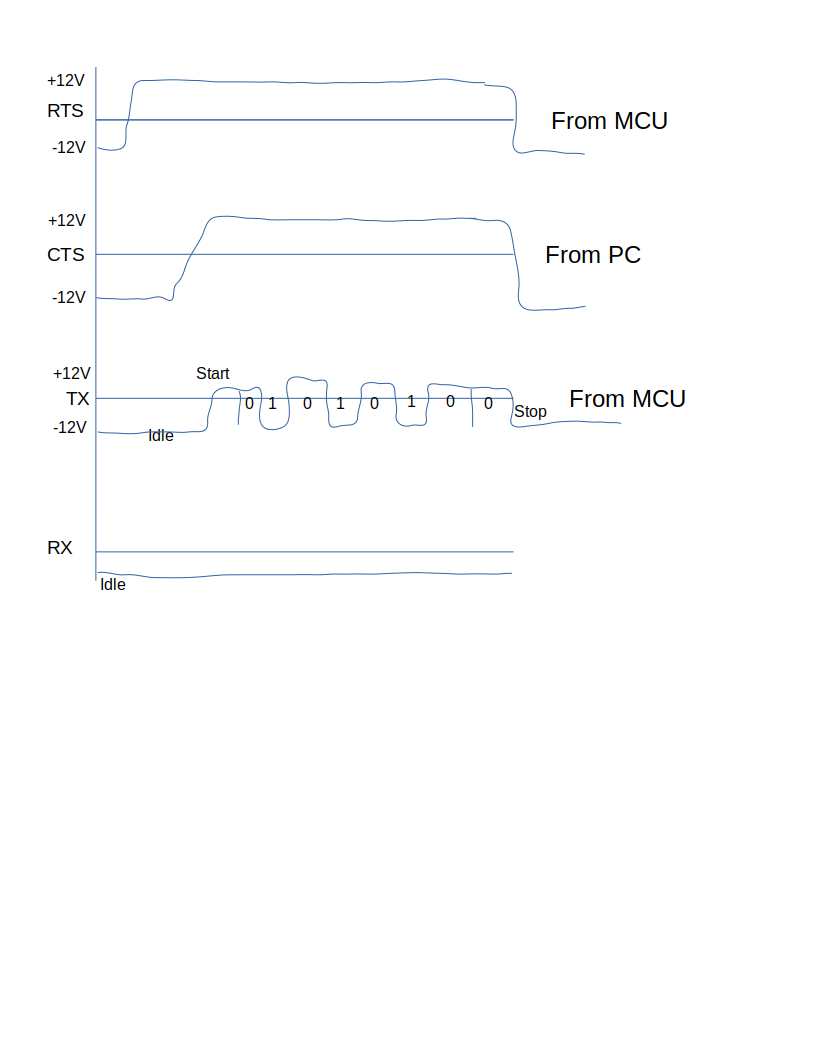
\includegraphics[scale=0.50]{HW1-1.png}
\item About 1/960 seconds for all 10 bits (8 bit char plus start, stop)
\end{enumerate}


\end{document}